\caulc
%E:\BAT-LATEX\MAIN-KIEM-TRA-THEO-2025\Khoi10\Data\10-GK1-03.tex
\begin{ex}
	Cho mệnh đề $P$: ``$15$ chia hết cho $3$''. Mệnh đề phủ định của mệnh đề $P$ là
	\choice
{$\overline{P}$: ``$15$ chia hết cho $6$''}
{$\overline{P}$: ``$15$ không chia hết cho $5$''}
{\True $\overline{P}$: ``$15$ không chia hết cho $3$''}
{$\overline{P}$: ``$15$ là số nguyên tố''}
\loigiai{
		Phủ định của khẳng định ``$15$ chia hết cho $3$'' là ``$15$ không chia hết cho $3$''.
	}
\end{ex}

%E:\BAT-LATEX\MAIN-KIEM-TRA-THEO-2025\Khoi10\Data\10-GK1-03.tex
\begin{ex}
	Hệ bất phương trình nào sau đây là hệ bất phương trình bậc nhất hai ẩn?
	\choice
{$\begin{cases} x - 2y \le 1 \\ x^2 + y > 0 \end{cases}$}
{$\begin{cases} x + 2y < 3 \\ y - z \ge 1 \end{cases}$}
{\True $\begin{cases} 2x + y - 3 \le 0 \\ x - 3y + 1 > 0 \end{cases}$}
{$\begin{cases} xy + 1 \ge 0 \\ x - y < 2 \end{cases}$}
\loigiai{
		Hệ $\begin{cases} 2x + y - 3 \le 0 \\ x - 3y + 1 > 0 \end{cases}$ gồm các bất phương trình bậc nhất hai ẩn $x, y$ nên là hệ bất phương trình bậc nhất hai ẩn.
	}
\end{ex}

%E:\BAT-LATEX\MAIN-KIEM-TRA-THEO-2025\Khoi10\Data\10-GK1-03.tex
\begin{ex}
	Số tập hợp con của tập hợp $S = \{a; b\}$ là
	\choice
{$1$}
{$3$}
{\True $4$}
{$2$}
\loigiai{
		Tập hợp gồm $2$ phần tử có số tập hợp con là $2^2 = 4$ (gồm: $\varnothing, \{a\}, \{b\}, \{a; b\}$).
	}
\end{ex}

%E:\BAT-LATEX\MAIN-KIEM-TRA-THEO-2025\Khoi10\Data\10-GK1-03.tex
\begin{ex}
	Cho tam giác $ABC$ có các cạnh $BC = a$, $CA = b$, $AB = c$. Mệnh đề nào sau đây là đúng?
	\choice
{$a^2 = b^2 + c^2 - 2bc \sin A$}
{\True $a^2 = b^2 + c^2 - 2bc \cos A$}
{$a^2 = b^2 + c^2 - bc \cos A$}
{$a^2 = b^2 + c^2 + 2bc \cos A$}
\loigiai{
		Theo định lí cosin trong tam giác $ABC$, ta có công thức: $a^2 = b^2 + c^2 - 2bc \cos A$.
	}
\end{ex}

%E:\BAT-LATEX\MAIN-KIEM-TRA-THEO-2025\Khoi10\Data\10-GK1-03.tex
\begin{ex}
	Trong các câu sau, câu nào là mệnh đề toán học?
	\choice
{Hôm nay thời tiết đẹp quá!}
{\True Tổng ba góc trong một tam giác bằng $180^\circ$}
{$2x + 1 > 0$}
{Bạn có thích học môn Toán không?}
\loigiai{
		Câu ``Tổng ba góc trong một tam giác bằng $180^\circ$'' là một khẳng định đúng về sự kiện toán học nên là một mệnh đề toán học. Các câu khác là câu cảm thán, câu hỏi hoặc mệnh đề chứa biến.
	}
\end{ex}

%E:\BAT-LATEX\MAIN-KIEM-TRA-THEO-2025\Khoi10\Data\10-GK1-03.tex
\begin{ex}
	Bất phương trình nào sau đây là bất phương trình bậc nhất hai ẩn?
	\choice
{$x + \dfrac{1}{y} \le 1$}
{$2x^2 + 3y \le 0$}
{\True $3x - 5y + 4 \ge 0$}
{$xy - 2 > 0$}
\loigiai{
		Bất phương trình bậc nhất hai ẩn có dạng $ax + by + c \ge 0$ (hoặc $>0, \le 0, <0$) với $a$ và $b$ không đồng thời bằng $0$. Do đó $3x - 5y + 4 \ge 0$ là bất phương trình bậc nhất hai ẩn.
	}
\end{ex}

%E:\BAT-LATEX\MAIN-KIEM-TRA-THEO-2025\Khoi10\Data\10-GK1-03.tex
\begin{ex}
	Cặp số nào sau đây là một nghiệm của bất phương trình $2x - 3y + 1 > 0$?
	\choice
{$(0; 1)$}
{$(-1; 1)$}
{\True $(2; 1)$}
{$(1; 2)$}
\loigiai{
		Thay cặp số $(2; 1)$ vào vế trái của bất phương trình: $2 \cdot 2 - 3 \cdot 1 + 1 = 2 > 0$ (đúng).\\
		Vậy $(2; 1)$ là một nghiệm của bất phương trình đã cho.
	}
\end{ex}

%E:\BAT-LATEX\MAIN-KIEM-TRA-THEO-2025\Khoi10\Data\10-GK1-03.tex
\begin{ex}
	Cho tam giác $ABC$ có các cạnh $a, b, c$ và $R, r, p$ lần lượt là bán kính đường tròn ngoại tiếp, nội tiếp và nửa chu vi của tam giác. Công thức nào sau đây tính diện tích $S$ của tam giác $ABC$?
	\choice
{$S = \dfrac{abc}{2R}$}
{$S = \dfrac{1}{2}ab \cos C$}
{\True $S = \dfrac{1}{2}bc \sin A$}
{$S = pR$}
\loigiai{
		Công thức tính diện tích tam giác theo hai cạnh và góc xen giữa là $S = \dfrac{1}{2}bc \sin A$.
	}
\end{ex}

%E:\BAT-LATEX\MAIN-KIEM-TRA-THEO-2025\Khoi10\Data\10-GK1-03.tex
\begin{ex}
	Tập hợp $A = \{x \in \mathbb{R} \mid -2 \le x < 5\}$ được viết dưới dạng khoảng, đoạn, nửa khoảng là
	\choice
{$(-2; 5)$}
{\True $[-2; 5)$}
{$(-2; 5]$}
{$[-2; 5]$}
\loigiai{
		Tập hợp các số thực thoả mãn $-2 \le x < 5$ là nửa khoảng $[-2; 5)$.
	}
\end{ex}

%E:\BAT-LATEX\MAIN-KIEM-TRA-THEO-2025\Khoi10\Data\10-GK1-03.tex
\begin{ex}
	Cho tập hợp $X = \{x \in \mathbb{N} \mid (x - 2)(x^2 - 9) = 0\}$. Viết tập hợp $X$ bằng cách liệt kê các phần tử ta được
	\choice
{\True $X = \{2; 3\}$}
{$X = \{-3; 2; 3\}$}
{$X = \{2\}$}
{$X = \{3\}$}
\loigiai{
		Phương trình $(x - 2)(x^2 - 9) = 0 \Leftrightarrow \left[\begin{array}{l} x = 2 \\ x = 3 \\ x = -3. \end{array}\right.$\\
		Vì $x \in \mathbb{N}$ nên ta nhận $x = 2$ và $x = 3$. Vậy $X = \{2; 3\}$.
	}
\end{ex}

%E:\BAT-LATEX\MAIN-KIEM-TRA-THEO-2025\Khoi10\Data\10-GK1-03.tex
\begin{ex}
	Cho mệnh đề $P$: ``$\forall x \in \mathbb{R}, x^2 + 1 > 0$''. Mệnh đề phủ định $\overline{P}$ của mệnh đề $P$ là
	\choice
{$\overline{P}$: ``$\exists x \in \mathbb{R}, x^2 + 1 < 0$''}
{\True $\overline{P}$: ``$\exists x \in \mathbb{R}, x^2 + 1 \le 0$''}
{$\overline{P}$: ``$\forall x \in \mathbb{R}, x^2 + 1 \le 0$''}
{$\overline{P}$: ``$\exists x \in \mathbb{R}, x^2 + 1 = 0$''}
\loigiai{
		Phủ định của mệnh đề ``$\forall x \in X, P(x)$'' là ``$\exists x \in X, \overline{P(x)}$''.\\
		Do đó phủ định của mệnh đề đã cho là ``$\exists x \in \mathbb{R}, x^2 + 1 \le 0$''.
	}
\end{ex}

%E:\BAT-LATEX\MAIN-KIEM-TRA-THEO-2025\Khoi10\Data\10-GK1-03.tex
\begin{ex}
	Giá trị của $\cos 120^\circ$ bằng
	\choice
{\True $-\dfrac{1}{2}$}
{$-\dfrac{\sqrt{3}}{2}$}
{$\dfrac{\sqrt{3}}{2}$}
{$\dfrac{1}{2}$}
\loigiai{
		Ta có $\cos 120^\circ = -\cos(180^\circ - 120^\circ) = -\cos 60^\circ = -\dfrac{1}{2}$.
	}
\end{ex}

\cauds
%E:\BAT-LATEX\MAIN-KIEM-TRA-THEO-2025\Khoi10\Data\10-GK1-03.tex
\begin{ex}
	Cho hệ bất phương trình bậc nhất hai ẩn $\begin{cases} x + y - 2 \le 0 \\ 2x - y + 2 \ge 0 \\ x \ge 0. \end{cases}$
	\choiceTF
{\True Miền nghiệm của hệ bất phương trình đã cho là một miền tam giác kể cả các cạnh của tam giác đó}
{\True Cặp số $(0; 0)$ là một nghiệm của hệ bất phương trình đã cho}
{\True Bất phương trình $x + y - 2 \le 0$ có bờ là đường thẳng đi qua hai điểm $(2; 0)$ và $(0; 2)$}
{Cặp số $(2; 1)$ là một nghiệm của hệ bất phương trình đã cho}
\loigiai{
		\begin{itemchoice}
			\itemch Đúng. Ba đường thẳng $x + y - 2 = 0$, $2x - y + 2 = 0$ và trục tung $x = 0$ cắt nhau tạo thành tam giác với các đỉnh $A(0; 2)$, $B(0; 2)$ trùng nhau hoặc ba giao điểm: $x = 0 \Rightarrow y = 2$; $x = 0 \Rightarrow y = 2$; và $x + y = 2, 2x - y = -2 \Rightarrow 3x = 0 \Rightarrow x = 0, y = 2$. Kết hợp miền $x \ge 0$ nằm giữa các đường thẳng, miền nghiệm tạo thành miền tam giác kín có biên.
		\itemch Đúng. Thay $(0; 0)$ vào hệ ta có: $\begin{cases} 0+0-2 = -2 \le 0 \\ 0-0+2 = 2 \ge 0 \\ 0 \ge 0 \end{cases}$ (thoả mãn).
			\itemch Đúng. Đường thẳng $d_1: x + y - 2 = 0$ cắt các trục toạ độ tại $(2; 0)$ và $(0; 2)$.
			\itemch Sai. Thay $(2; 1)$ vào bất phương trình đầu tiên: $2 + 1 - 2 = 1 \le 0$ (vô lý). Do đó $(2; 1)$ không là nghiệm của hệ.
			\end{itemchoice}
	}
\end{ex}

%E:\BAT-LATEX\MAIN-KIEM-TRA-THEO-2025\Khoi10\Data\10-GK1-03.tex
\begin{ex}
	Cho tam giác $ABC$ có góc $\widehat{B} = 60^\circ$, $\widehat{C} = 45^\circ$ và cạnh $AC = b = 6\sqrt{2}$. Gọi $R$ là bán kính đường tròn ngoại tiếp của tam giác $ABC$.
	\choiceTF
{\True Theo định lí sin, ta có đẳng thức $\dfrac{a}{\sin A} = \dfrac{b}{\sin B} = \dfrac{c}{\sin C} = 2R$}
{Góc $\widehat{A} = 75^\circ$ và độ dài cạnh $BC = 2\sqrt{6} + 2\sqrt{2}$}
{Bán kính đường tròn ngoại tiếp tam giác $ABC$ là $R = 4\sqrt{3}$}
{\True Độ dài cạnh $AB$ bằng $4\sqrt{3}$}
\loigiai{
		\begin{itemchoice}
			\itemch Đúng. Đây là công thức của định lí sin.
			\itemch Sai. Ta có $\widehat{A} = 180^\circ - (60^\circ + 45^\circ) = 75^\circ$.\\
			$a = BC = 2R \cdot \sin 75^\circ = 4\sqrt{6} \cdot \left(\dfrac{\sqrt{6} + \sqrt{2}}{4}\right) = 6 + 2\sqrt{3} \ne 2\sqrt{6} + 2\sqrt{2}$.
		\itemch Sai. Theo định lí sin: $2R = \dfrac{b}{\sin B} = \dfrac{6\sqrt{2}}{\sin 60^\circ} = \dfrac{6\sqrt{2}}{\frac{\sqrt{3}}{2}} = 4\sqrt{6} \Rightarrow R = 2\sqrt{6}$.
			\itemch Đúng. Ta có cạnh $AB = c$. Theo định lí sin: $\dfrac{c}{\sin C} = 2R \Rightarrow c = 2R \cdot \sin 45^\circ = 4\sqrt{6} \cdot \dfrac{\sqrt{2}}{2} = 4\sqrt{3}$.
			\end{itemchoice}
	}
\end{ex}
\caukq
%E:\BAT-LATEX\MAIN-KIEM-TRA-THEO-2025\Khoi10\Data\10-GK1-03.tex
\begin{ex}
	Cho mệnh đề chứa biến $P(n)\colon ``2n^2 + 5n - 12 \le 0"$ với $n$ là số nguyên. Có bao nhiêu giá trị của $n$ để mệnh đề $P(n)$ là mệnh đề đúng?
	\loigiai{
		Mệnh đề $P(n)$ đúng khi và chỉ khi:
		\[
		2n^2 + 5n - 12 \le 0
		\]
		Xét tam thức bậc hai $f(n) = 2n^2 + 5n - 12$:
		\begin{itemize}
			\item Có hai nghiệm phân biệt: $n = \dfrac{3}{2}$ và $n = -4$.
			\item Hệ số $a = 2 > 0$.
		\end{itemize}
		Do đó, bất phương trình $2n^2 + 5n - 12 \le 0$ có tập nghiệm là:
		\[
		-4 \le n \le \dfrac{3}{2}
		\]
		Vì $n$ là số nguyên ($n \in \mathbb{Z}$) nên $n \in \{-4; -3; -2; -1; 0; 1\}$.
		
		Vậy có tất cả $6$ giá trị nguyên của $n$ để mệnh đề chứa biến $P(n)$ là một mệnh đề đúng.
	}
\end{ex}

%E:\BAT-LATEX\MAIN-KIEM-TRA-THEO-2025\Khoi10\Data\10-GK1-03.tex
\begin{ex}
	Cho tam giác $ABC$ có cạnh $AB = 6$, $AC = 8$ và góc $\widehat{A} = 30^\circ$. Tính diện tích của tam giác $ABC$.
	\shortans[]{12}
	\loigiai{
		Diện tích tam giác $ABC$ là:\\
		$S = \dfrac{1}{2}AB \cdot AC \cdot \sin A = \dfrac{1}{2} \cdot 6 \cdot 8 \cdot \sin 30^\circ = \dfrac{1}{2} \cdot 48 \cdot \dfrac{1}{2} = 12$.
	}
\end{ex}

%E:\BAT-LATEX\MAIN-KIEM-TRA-THEO-2025\Khoi10\Data\10-GK1-03.tex
\begin{ex}
	Cho tam giác $ABC$ có $b = 7$, $c = 5$ và $\cos A = \dfrac{3}{5}$. Tính độ dài cạnh $a$ của tam giác $ABC$.
	\shortans[]{5.66}
	\loigiai{
		Áp dụng định lí cosin trong tam giác $ABC$:\\
		$a^2 = b^2 + c^2 - 2bc \cos A = 7^2 + 5^2 - 2 \cdot 7 \cdot 5 \cdot \dfrac{3}{5} = 49 + 25 - 42 = 32$.\\
		Suy ra $a = \sqrt{32} = 4\sqrt{2} \approx 5.66$.
	}
\end{ex}

%E:\BAT-LATEX\MAIN-KIEM-TRA-THEO-2025\Khoi10\Data\10-GK1-03.tex
\begin{ex}
	Cho tập hợp $A = \{x \in \mathbb{Z} \mid -3 \le 2x - 1 < 7\}$. Tập hợp $A$ có bao nhiêu phần tử?
	\shortans[]{5}
	\loigiai{
		Ta có: $-3 \le 2x - 1 < 7 \Leftrightarrow -2 \le 2x < 8 \Leftrightarrow -1 \le x < 4$.\\
		Vì $x \in \mathbb{Z}$ nên $x \in \{-1; 0; 1; 2; 3\}$.\\
		Tập hợp $A$ có $5$ phần tử.
	}
\end{ex}
\cauTL
%E:\BAT-LATEX\MAIN-KIEM-TRA-THEO-2025\Khoi10\Data\10-GK1-03.tex
\begin{ex}
	Một cơ sở thủ công mỹ nghệ sản xuất hai loại giỏ mây gồm loại $A$ và loại $B$. Để sản xuất một chiếc giỏ loại $A$ cần $2\text{ kg}$ sợi mây và $3\text{ giờ}$ gia công. Để sản xuất một chiếc giỏ loại $B$ cần $3\text{ kg}$ sợi mây và $2\text{ giờ}$ gia công. Cơ sở hiện dự trữ tối đa $24\text{ kg}$ sợi mây và tổng quỹ thời gian của thợ không vượt quá $24\text{ giờ}$. Mỗi chiếc giỏ loại $A$ bán được lãi $80\,000\text{ đồng}$, mỗi chiếc giỏ loại $B$ bán được lãi $90\,000\text{ đồng}$. Tìm phương án sản xuất mỗi loại giỏ sao cho tổng tiền lãi thu được lớn nhất.
	\loigiai{
		Gọi $x, y$ lần lượt là số giỏ mây loại $A$ và loại $B$ mà cơ sở sản xuất ($x, y \in \mathbb{N}$).\\
		Hệ bất phương trình ràng buộc lượng nguyên liệu và thời gian hoàn thành là:
		\[
		\begin{cases}
		2x + 3y \le 24 \\
		3x + 2y \le 24 \\
		x \ge 0 \\
		y \ge 0.
		\end{cases}
		\]
		Miền nghiệm của hệ bất phương trình là miền tứ giác $OABC$ (kể cả biên) với toạ độ các đỉnh:
		\begin{itemize}
			\item Gốc toạ độ $O(0; 0)$;
			\item Điểm $A(8; 0)$ là giao điểm của đường thẳng $3x + 2y = 24$ với trục hoành;
			\item Điểm $B$ là giao điểm của hai đường thẳng $2x + 3y = 24$ và $3x + 2y = 24$. Toạ độ $B$ là nghiệm hệ:
			\[
			\begin{cases} 2x + 3y = 24 \\ 3x + 2y = 24 \end{cases} \Leftrightarrow \begin{cases} x = \dfrac{24}{5} = 4{,}8 \\ y = \dfrac{24}{5} = 4{,}8 \end{cases} \implies B\left(\dfrac{24}{5}; \dfrac{24}{5}\right);
			\]
			\item Điểm $C(0; 8)$ là giao điểm của đường thẳng $2x + 3y = 24$ với trục tung.
		\end{itemize}
		\begin{center}
			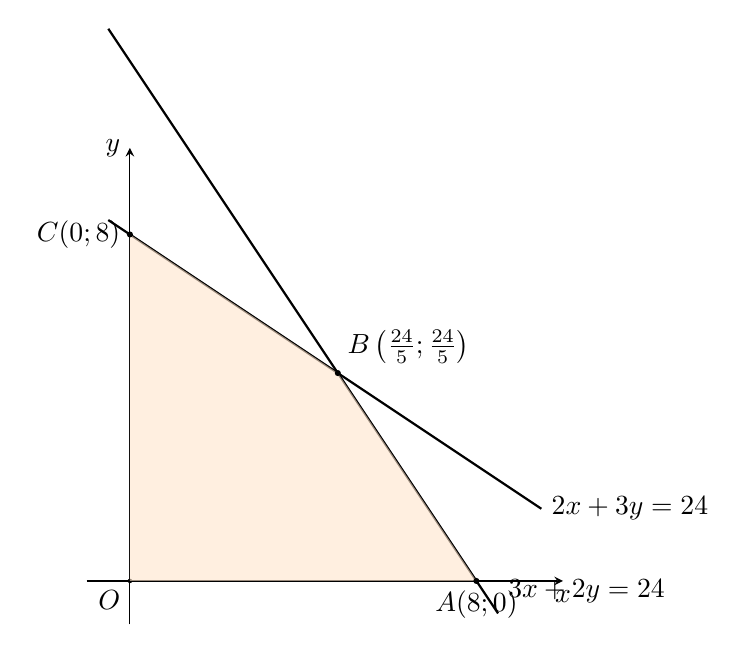
\begin{tikzpicture}[scale=0.55,>=stealth]
			\draw[->] (-1,0) -- (10,0) node[below] {$x$};
			\draw[->] (0,-1) -- (0,10) node[left] {$y$};
			\fill (0,0) circle (1.5pt) node[below left] {$O$};
			\draw[thick,domain=-0.5:8.5] plot (\x,{12 - 1.5*\x}) node[above right] {$3x + 2y = 24$};
			\draw[thick,domain=-0.5:9.5] plot (\x,{8 - 2/3*\x}) node[right] {$2x + 3y = 24$};
			\fill[orange!20,opacity=0.6] (0,0) -- (8,0) -- (4.8,4.8) -- (0,8) -- cycle;
			\fill (8,0) circle (2pt) node[below] {$A(8;0)$};
			\fill (4.8,4.8) circle (2pt) node[above right] {$B\left(\frac{24}{5};\frac{24}{5}\right)$};
			\fill (0,8) circle (2pt) node[left] {$C(0;8)$};
			\end{tikzpicture}
		\end{center}
		Tổng số tiền lãi thu về tính theo hàm mục tiêu:
		\[
		F(x; y) = 80x + 90y \quad (\text{nghìn đồng}).
		\]
		Do $x, y \in \mathbb{N}$, các điểm nguyên $(x; y)$ nằm trong tứ giác $OABC$ gần đỉnh $B(4{,}8; 4{,}8)$ được khảo sát:
		\begin{itemize}
			\item Với $(x; y) = (4; 4)$:
			\[
			\begin{cases} 2(4) + 3(4) = 20 \le 24 \\ 3(4) + 2(4) = 20 \le 24 \end{cases} \implies F(4; 4) = 80\cdot 4 + 90\cdot 4 = 680 \text{ nghìn đồng}.
			\]
			\item Với $(x; y) = (5; 4)$:
			\[
			\begin{cases} 2(5) + 3(4) = 22 \le 24 \\ 3(5) + 2(4) = 23 \le 24 \end{cases} \implies F(5; 4) = 80\cdot 5 + 90\cdot 4 = 760 \text{ nghìn đồng}.
			\]
			\item Với $(x; y) = (4; 5)$:
			\[
			\begin{cases} 2(4) + 3(5) = 23 \le 24 \\ 3(4) + 2(5) = 22 \le 24 \end{cases} \implies F(4; 5) = 80\cdot 4 + 90\cdot 5 = 770 \text{ nghìn đồng}.
			\]
			\item Kiểm tra thêm các đỉnh biên:
			\begin{itemize}
				\item $A(8; 0) \implies F(8; 0) = 80 \cdot 8 + 0 = 640\text{ nghìn đồng}$.
				\item $C(0; 8) \implies F(0; 8) = 0 + 90 \cdot 8 = 720\text{ nghìn đồng}$.
				\item Cặp $(3; 6)$: $2(3) + 3(6) = 24 \le 24$, $3(3) + 2(6) = 21 \le 24 \implies F(3; 6) = 80\cdot 3 + 90\cdot 6 = 780\text{ nghìn đồng}$.
				\item Cặp $(2; 6)$: $F(2; 6) = 700\text{ nghìn đồng} < 780$.
				\item Cặp $(3; 7)$: $2(3) + 3(7) = 27 > 24$ (loại).
			\end{itemize}
		\end{itemize}
		So sánh tất cả các phương án nguyên, giá trị tiền lãi cao nhất đạt được là $F(3; 6) = 780\text{ nghìn đồng}$.\\
		Vậy cơ sở nên sản xuất $3$ chiếc giỏ loại $A$ và $6$ chiếc giỏ loại $B$ để đạt lợi nhuận lớn nhất là $780\,000\text{ đồng}$.
	}
\end{ex}

%D:\BAT-LATEX\MAIN-KIEM-TRA-THEO-2025\Khoi10\Data\0-CD\de-giua-ky-1-lop10-2025-2026-TRUONG.tex
\begin{ex}%[2025-K10-SangtacdeGKI]%[ChuongtrinhCD, Trần Lê Tuấn Anh]%[0H5V2-6]
	Tìm $A \cap B$, $A \cup B$ và $A \setminus B$ biết $A=\{x\in\mathbb{R}\mid  x \leq 2\}, B=\{x \in \mathbb{R} \mid -3 < x \leq 8\}$
	\loigiai{
		Ta biểu diễn các tập hợp dưới dạng khoảng, đoạn:
		$A = (-\infty; 2]$;		$B = (-3; 8]$
		
		Ta có:
		\begin{itemize}
			\item Phép giao: $A \cap B = \{x \in \mathbb{R} \mid x \leq 2 \text{ và } -3 < x \leq 8\} = (-3; 2]$.
			\item Phép hợp: $A \cup B = \{x \in \mathbb{R} \mid x \leq 2 \text{ hoặc } -3 < x \leq 8\} = (-\infty; 8]$.
			\item Phép hiệu: $A \setminus B = (-\infty; -3]$.
		\end{itemize}
	}
	%<MyLT2>
\end{ex}

%E:\BAT-LATEX\MAIN-KIEM-TRA-THEO-2025\Khoi10\Data\10-GK1-03.tex
\begin{ex}
	Để đo chiều cao của một tòa nhà mà không thể tiếp cận trực tiếp chân tòa nhà (do khuôn viên có hàng rào bao quanh), một nhóm học sinh đặt giác kế tại hai điểm $A$ và $B$ trên mặt đất bằng phẳng, cách nhau một khoảng $AB = 30\text{ m}$ cùng hướng về tòa nhà. Gọi đỉnh tòa nhà là điểm $C$ và chân tòa nhà trên mặt đất là điểm $D$ ($CD$ vuông góc với mặt đất tại $D$, với các điểm $A, B, D$ thẳng hàng).
	
	Qua giác kế, nhóm học sinh đo được góc nâng nhìn lên đỉnh tòa nhà từ điểm $A$ là $\widehat{CAD} = 32^\circ$ và từ điểm $B$ là $\widehat{CBD} = 48^\circ$. Coi chiều cao của giác kế đặt tại $A$ và $B$ không đáng kể. 
	\begin{enumerate}[a)]
		\item Tính số đo góc $\widehat{ACB}$ và độ dài đoạn thẳng $BC$ (làm tròn kết quả đến hàng phần mười của mét).
		\item Tính chiều cao $CD$ của tòa nhà (làm tròn kết quả đến hàng phần mười của mét).
	\end{enumerate}
	\loigiai{
		\begin{center}
			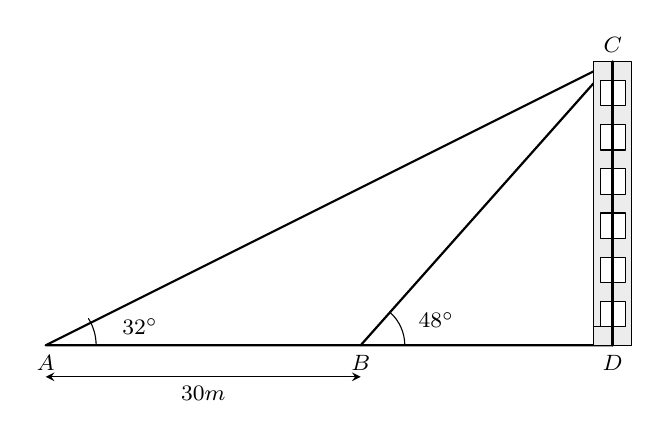
\begin{tikzpicture}[scale=0.8, font=\footnotesize, line join=round, line cap=round, >=stealth]
			% Toa do
			\coordinate (D) at (0,0);
			\coordinate (C) at (0,4.5);
			\coordinate (B) at (-4,0);
			\coordinate (A) at (-9,0);
			
			% Ve hinh
			\draw[thick] (A) -- (D) -- (C) -- cycle;
			\draw[thick] (C) -- (B);
			
			% Toa nha (minh hoa)
			\draw[fill=gray!15] (-0.3,0) rectangle (0.3,4.5);
			\foreach \y in {0.5, 1.2, 1.9, 2.6, 3.3, 4.0} {
				\draw[fill=white] (-0.2,\y-0.2) rectangle (0.2,\y+0.2);
			}
			\draw[line width=1pt] (D) -- (C);
			
			% Goc vuong
			\draw (0,0.3) -- (-0.3,0.3) -- (-0.3,0);
			
			% Ky hieu goc
			\draw (-8.2,0) arc (0:32:0.8);
			\node at (-7.5,0.3) {$32^\circ$};
			\draw (-3.3,0) arc (0:48:0.7);
			\node at (-2.8,0.4) {$48^\circ$};
			
			% Kich thuoc AB
			\draw[<->] (-9,-0.5) -- (-4,-0.5) node[midway, below] {$30\text{ m}$};
			
			% Ten diem
			\node[below] at (A) {$A$};
			\node[below] at (B) {$B$};
			\node[below] at (D) {$D$};
			\node[above] at (C) {$C$};
			\end{tikzpicture}
		\end{center}
		
		\begin{enumerate}[a)]
			\item \textbf{Tính số đo góc $\widehat{ACB}$ và độ dài đoạn thẳng $BC$:}
			
			Vì ba điểm $A, B, D$ thẳng hàng theo thứ tự đó nên góc $\widehat{CBD}$ là góc ngoài tại đỉnh $B$ của tam giác $ABC$. Do đó:
			$$\widehat{CBD} = \widehat{CAB} + \widehat{ACB} \implies \widehat{ACB} = \widehat{CBD} - \widehat{CAB} = 48^\circ - 32^\circ = 16^\circ.$$
			
			Áp dụng định lý sin trong tam giác $ABC$, ta có:
			$$\frac{BC}{\sin \widehat{BAC}} = \frac{AB}{\sin \widehat{ACB}} \implies BC = \frac{AB \cdot \sin \widehat{BAC}}{\sin \widehat{ACB}}.$$
			
			Thay số:
			$$BC = \frac{30 \cdot \sin 32^\circ}{\sin 16^\circ} \approx \frac{30 \cdot 0{,}5299}{0{,}2756} \approx 57{,}7\text{ m}.$$
			
			\item \textbf{Tính chiều cao $CD$ của tòa nhà:}
			
			Xét tam giác $BCD$ vuông tại $D$, ta có:
			$$CD = BC \cdot \sin \widehat{CBD}.$$
			
			Thay giá trị $BC$ vừa tính được vào:
			$$CD = 57{,}7 \cdot \sin 48^\circ \approx 57{,}7 \cdot 0{,}7431 \approx 42{,}9\text{ m}.$$
			
			Vậy chiều cao của tòa nhà xấp xỉ $42{,}9\text{ m}$.
		\end{enumerate}
	}
\end{ex}
\Closesolutionfile{ans}
\Closesolutionfile{ansbook}

\hetde
\label{3281}

\newpage
\begin{dapanMyLT}
\setcounter{page}{1}
\rfoot{Trang \thepage/\pageref{DA3281} $-$ Đáp án mã đề 3281}
\begin{center}
\bf ĐÁP ÁN PHẦN TRẮC NGHIỆM 4 PHƯƠNG ÁN - MÃ ĐỀ 3281\vspace{12pt}
\inputansbox[1]{10}{ans/ansMyLTTN3281}
\end{center}
\begin{center}
\bf ĐÁP ÁN PHẦN TRẮC NGHIỆM ĐÚNG SAI - MÃ ĐỀ 3281
\end{center}
\inputansbox[2]{3}{ans/ansMyLTTF3281}
\begin{center}
\bf ĐÁP ÁN PHẦN TRẢ LỜI NGẮN - MÃ ĐỀ 3281
\end{center}
\inputansbox[3]{6}{ans/ansMyLTSA3281}
\label{DA3281}
\begin{center}
\bf ĐÁP ÁN PHẦN TỰ LUẬN MÃ ĐỀ 3281
\end{center}
\input{ans/ansbookMyLTTL3281}
\clearpage
\end{dapanMyLT}

\end{document}

